\chapter{可信计算技术与近来深度学习与密码学}
\label{chap:4}

本章针对可信计算技术与近来深度学习与密码学等进来资讯进行整理。当中共分为可信计算技术与深度学习两大部分进行说明。

\section{可信计算概述}

\subsection{为何需要可信计算}

如今信息技术已经成为了人们生活中不可分割的一部分,人们每天都通过计算机和互联网获取信息、进行各种活动。但计算机与网络空间并不总是安全的,一方面黑客们会通过在网络中散布恶意病毒来对正常用户进行攻击,例如2017年5月爆发的勒索病毒;另一方面许多不良厂商会在自己的软件中“开后门”,趁用户不注意时获取用户的隐私或者弹出弹窗广告,这些都给维护网络空间的信息安全带来了巨大的挑战。为了使人们能够正常地通过计算机在互联网上进行各种活动,我们必须建立一套安全、可靠的防御体系来确保我们的计算机能够按照预期稳定地提供服务。

目前多数的网络安全系统主要由防火墙、入侵检测、病毒防范等组成。这种常规的安全手段只能在网络层、边界层设防,在外围对非法用户和越权访问进行封堵,以达到防止外部攻击的目的。由于这些安全手段缺少对访问者源端—客户机的控制,加之操作系统的不安全导致应用系统的各种漏洞层出不穷,其防护效果正越来越不理想。此外,封堵的办法是捕捉黑客攻击和病毒入侵的特征信息,而这些特征是已发生过的滞后信息,属于“事后防御”。随着恶意用户的攻击手段变化多端,防护者只能把防火墙越砌越高、入侵检测越做越复杂、恶意代码库越做越大,误报率也随之增多,使得安全的投入不断增加,维护与管理变得更加复杂和难以实施,信息系统的使用效率大大降低,而对新的攻击毫无防御能力。近年来,“震网”“火焰”“Mirai”“黑暗力量”“WannaCry勒索病毒”等重大安全事件频频发生,显然,传统防火墙、入侵检测、病毒防范等“老三样”封堵查杀的被动防御已经过时,网络空间安全正遭遇严峻挑战。安全防护手段在终端架构上缺乏控制,这是一个非常严重的安全问题,难以应对利用逻辑缺陷的攻击。目前利用逻辑缺陷的漏洞频繁爆出,如“幽灵”“熔断”,都是因为CPU性能优化机制存在设计缺陷,只考虑了提高计算性能而没有考虑安全性。由这种底层设计缺陷导致的漏洞难以修补,即使有了补丁其部署难度也是越来越大。幽灵、熔断的补丁部署后会使性能下降3 0\%。补丁难打、漏洞难防已经是当前信息安全防御主要问题之一。

可信计算正是为了解决计算机和网络结构上的不安全,从根本上提高安全性的技术方法,可信计算是从逻辑正确验证、计算体系结构和计算模式等方面的技术创新,以解决逻辑缺陷不被攻击者所利用的问题,形成攻防矛盾的统一体,确保完成计算任务的逻辑组合不被篡改和破坏,实现正确计算。

\subsection{何为是可信计算}

可信计算概念最早可以追溯到美国国防部颁布的TCSEC准则。1983年美国国防部制定了世界上第一个《可信计算机系统评价标准》(TCSEC),第一次提出了可信计算机和可信计算基(Trusted Computing Base,TCB)的概念,并把TCB作为系统系统安全的基础。

\subsubsection{可信的定义}

可信计算的首要问题是要回答什么是可信。目前关于可信尚未形成统一的定义,不同的专家和不同的组织机构有不同的解释。主要有以下几种说法。1990年,国际标准化组织与国际电子技术委员会ISO/IEC在其发布的目录服务系列标准中基于行为预期性定义了可信性:如果第2个实体完全按照第1个实体的预期行动时,则第1个实体认为第2个实体 是可信的。1999年,国际标准化组织与国际电子技术委员会在ISO/IEC15408标准中定义可信为:参与计算的组件、操作或过程在任意的条件下是可预测的,并能够抵御病毒和一定程度的物理干扰。2002年,TCG用实体行为的预期性来定义可信:一个实体是可信的,如果它的行为总是以预期的方式,朝着预期的目标。这一定义的优点是抓住了实体的行为特征,符合哲学上实践是检验真理的唯一标准的基本原则。IEEE可信计算技术委员会认为,可信是指计算机系统所提供的服务是可信赖的,而且这种可信赖是可论证的。

\subsubsection{信任的获得方法}

信任的获得方法主要有直接和间接两种。设A和B以前有过交往,则A对B的可信度可以通常考察B以往的表现来确定,我们称这种通过直接交往得到的信任值为直接信任值。设A和B以前没有任何交往,但A信任C,并且C信任B,那么此时我们称A对B的信任为间接信任。有时还可能出现多级间接信任的情况,这时便产生了信任链。

\subsubsection{可信计算的基本思想}

在计算平台中,首先创建一个安全信任根,再建立从硬件平台、操作系统到应用系统的信任链,在这条信任链上从根开始一级测量认证一级,一级信任一级,以此实现信任的逐级扩展,从而构建一个安全可信的计算环境。一个可信计算系统由信任根、可信硬件平台、可信操作系统和可信应用组成,其目标是提高计算平台的安全性。

\subsection{可信计算的发展概况}

早在20世纪60年代,为了提高硬件设备的安全性,人们设计了具有高可靠性的可信电路,可信的概念开始萌芽。到20世纪70年代初期,Anderson首次提出来了可信系统的概念,为美国后续的TCSEC(彩虹系列),可信计算机、可信计算基(TCB)、可信网络、可信数据库等的提出奠定了基础。彩虹系列是最早的一套可信计算技术文件,标志着可信计算的出现,也使系统的可信不断丰富可信的内涵,可信计算的理念和标准初具雏形。

从 20 世纪 90 年代开始,随着科学计算研究的体系化不断规范、规模的逐步扩大,可信计算产业组织和标准逐步形成体系并完善。1999年, IBM、HP、Intel和微软等著名IT企业发起成立了可信计算平台联盟(TCPA, Trusted Computing Platform Alliance),这标志着可信计算进入产业界。2003年,TCPA 改组为可信计算组织(TCG, Trusted Computing Group)。目前,TCG已经制定了一系列的可信计算技术规范,如可信PC、可信平台模块(TPM)、可信软件栈(TSS)、可信网络连接(TNC)、可信手机模块等,且不断地对这些技术规范进行修改完善和版本升级。

早在 2000 年伊始,我国就开始关注可信计算,并进行了立项、研究,和国外不同,我国在可信计算上走的是先引进技术后自主研发、先产品化后标准化的跨越式发展。2004 年,武汉瑞达生产了中国第一款TPM,之后联想、长城等基于TPM生产了可信PC。2005年1月,全国信息安全标准化技术委员会成立了可信计算工作小组(WGI),先后研制制定了可信密码模块(TCM)、可信主板、可信网络联接等多项标准规范。2005年,国家出台“十一五”规划和“863”计划,把“可信计算”列入重点支持项目,我国出现了一系列的可信计算产品。截止到目前,国际上已形成以 TPM 芯片为信任根的TCG标准系列,国内已形成以 TCM 芯片为信任根的双体系架构可信标准系列。其国际与中国国内两套标准最主要差异如下所列。

\begin{itemize}
\item [1.] 信任芯片是否支持国产密码算法,国家密码局主导提出了中国商用密码可信计算应用标准,并禁止加载国际算法的可信计算产品在国内销售。
\item [2.]信任芯片是否支持板卡层面的优先加电控制,国内部分学者认为国际标准提出的CPU先加电、后依靠密码芯片建立信任链的模式强度不够,为此,提出基于TPCM芯片的双体系计算安全架构,TPCM 芯片除了密码功能外,必须先于 CPU 加电,先于CPU对BIOS进行完整性度量。
\item [3.] 可信软件栈是否支持操作系统层面的透明可信控制,国内部分学者认为国际标准需要程序被动调用可信接口,不能在操作系统层面进行主动度量,为此,提出在操作系统内核层面对应用程序完整性和程序行为进行透明可信判定及控制思路。
\end{itemize}

\subsection{可信计算技术}

\subsubsection{信任根}

TCG 定义的信任根包括 3 个根,其包含负责完整性度量的可信度量根(RTM),负责报告信任根的可信报告根(RTR),负责存储信任根的可信存储根(RTS)。其中,RTM 是一个软件模块、RTR 是由 TPM 的平台配置寄存器(PCR)和背书密钥(EK)组成、RTS是由TPM的PCR和存储根密钥(SRK)组成。实践中,RTM 在构建信任链的过程中,将完整性度量形成的信息传递给 RTS,RTS 使用 TPM 的平台配置寄存器存放度量扩展值、使用TPM提供的密码学服务保护度量日志。 RTR 主要用于远程证明过程,向实体提供平台可信状态信息,主要内容包括平台配置信息、审计日志与一般由背书密钥或者基于背书密钥保护的身份密钥承担的身份密钥。

\subsubsection{信任链}

信任链的主要作用是将信任关系扩展到整个计算机平台,它建立在信任根的基础上。信任链可以通过可信度量机制来获取各种各样影响平台可信性的数据,并通过将这些数据与预期数据进行比较,来判断平台的可信性。建立信任链时遵循以下 3 条规则。

\begin{itemize}
\item [1.] 所有模块或组件,除了 CRTM,也就是信任链构建起点,第一段运行的用于可信度量的代码,在没有经过度量以前,均认为是不可信的。同时,只有通过可信度量且与预期数据相符的模块或组件,才可归入可信边界内。
\item [2.] 可信边界内部的模块或组件,可以作为验证代理,对尚未完成验证的模块或组件进行完整性验证。
\item [3.] 只有可信边界内的模块或组件,才可以获得相关的 TPM 控制权,可信边界以外的模块或组件无法控制或使用可信平台模块。
\end{itemize}

\begin{figure}[htb]
\centering 
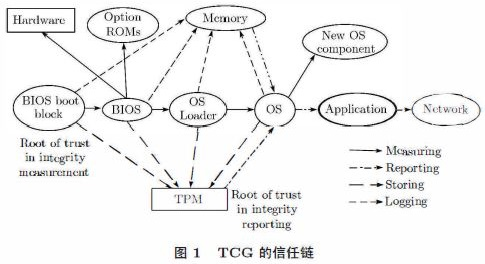
\includegraphics[width=0.90\textwidth]{img/ch3m1.jpg} 
\caption{TCG 信任链}
\label{Test}
\end{figure}

TCG 的 可信 PC 技术规范中提出了可信PC中的信任链,如图中所示,TCG的信任链很好地体现了度量存储报告机制。即对平台可行性进行度量,对度量的可信值进行存储。另外名词解释如下所示 :

\begin{itemize}
\item [1.] 度量 : 该信任链以 BIOS 引导区与TPM为信任根,其中 BIOS 引导区为可信度量根(RTM),TPM为可信存储根(RTS)、可信报告根(RTR)。从BIOS引导区出发,到OS Loader、再到 OS、应用,构成一条信任链。沿着这条信任链,一级度量一级,一级信任一级,确保平台资源的完整性。
\item [2.] 存储 : 由于可信平台模块存储空间有限,所以采用度量扩展的方法即现有度量值和新度量值相连再次散列来记录和存储度量值到可信平台模块的 PC中,同时将度量对象的详细信息和度量结果作为日志存储在磁盘中。存储在磁盘中的度量日志和存储在 PCR 中的度量值是相互印证的,防止磁盘中的日志被篡改。
\item [3.] 报告 : 度量、存储之后,当访问客体询问时,可以提供报告,供访问对象判断平台的可信状态。向客体提供的报告内容包括PCR值和日志。为了确保报告内容的安全,还须采用加密、数字签名和认证技术,这一功能被称为平台远程证明。
\end{itemize}

\subsubsection{可信平台模块}

目前主要的可信平台模块主要有三种,分别是 TCG 的 TPM、中国的 TCM 和 TPCM,本小节只介绍 TCG 的 TPM。可信平台模块是可信计算平台的信任根的 RTS、RTR,它本身是一个 SOC 芯片,由 CPU、存储器、I/O、密码协处理器、随机数产生器和嵌入式操作系统等部件组成,主要用于可信度量的存储、可信度量的报告、密钥产生、加密和签名、数据安全存储等功能。

TCG 先后发布过多个版本的TPM标准,其中,TPM 1.2 使用较为广泛,但随着信息计算机技术的不断发展,TPM 1.2无 法满足新技术下的需求,2014 TCG 发布了TPM 2.0,相较于 TPM 1.2,TPM 2.0有如下改进,(1) 吸收原有 TPM (TPM1.2) 和中国 TCM 的优点、(2) 改进原 TPM 在密码算法灵活方面存在的问题、(3) 使之成为一个国际标准,解决不同国家的本地需求,并保持较好的兼容性,如中国国内的 TPM 2.0 芯片支持国家密码局允许的密码学算法 SM3、SM2、SM4 等。 TPM 2.0结构及模块功能如图所示。

\begin{figure}[htb]
\centering 
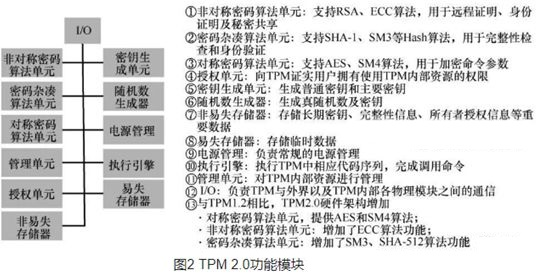
\includegraphics[width=0.90\textwidth]{img/ch3m2.jpg} 
\caption{TPM 2.0}
\label{Test}
\end{figure}

\subsubsection{可信支撑软件}

可信支撑软件是操作系统层面安全应用可以调用可信计算平台提供的可信服务接口,从而为用户提供可信服务。TCG Software Stack (TSS) 是可信计算平台上TPM的支撑软件,其 TSS 的作用主要是为操作系统和应用软件提供使用 TPM 的接口。目前,TSS 主要有 TSS 1.2 和 TSS 2.0 两个版本。其中基于 TPM 2.0 的 TSS 2.0 是最新的版本,其结构如下图所示。此外開放授權原始碼可於 GitHub 項目平台,名為 tpm2-software/tpm2-tss 找到。

\begin{figure}[htb]
\centering 
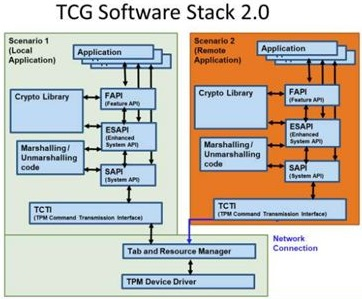
\includegraphics[width=0.90\textwidth]{img/ch3m3.jpg} 
\caption{TCG Software Stack}
\label{Test}
\end{figure}


\subsection{围绕可信计算的一些争议}

尽管可信计算一经提出就获得了众多学者的大力支持,但可信计算的反对者指出:保护计算机不受病毒和攻击者影响的安全机制,同样会限制其属主的行为。剑桥大学的密码学家Ross Anderson他们指出这将使得强制性垄断成为可能,从而会伤害那些购买可信计算机的人们。Anderson还总结道"最根本的问题在于控制可信计算基础设施的人将获取巨大的权力。拥有这样的权力就像是可以迫使所有人都使用同一个银行、同一个会计或同一个律师。而这种权力能以多种形式被滥用。

除此之外,由于装有可信计算设备的计算机可以唯一证明自己的身份,厂商或其他可以使用证明功能的人就能够以非常高的可能性确定用户的身份。可信计算的赞成者指出,它可以使在线购物和信用卡交易更安全,但这可能导致计算机用户失去访问互联网时希望拥有的匿名性。批评者指出这可能导致对政治言论自由,新闻记者使用匿名信息源,揭发政治博客,以及其他公众需要通过匿名性来防止报复的领域,产生抑制作用。

\section{深度学习与密码学}

加密领域是资安攻防的一大重点,举凡 RSA、AES、DES、Blowfish 和 Twofish 这些,都是著名的加密演算法,而这些演算法,可以让攻击者花较多时间破解,并配合验证机制以减少资料库被盗取的机会。在人工智慧开始流行之后,也渐渐开始出现能以机器学习、深度学习实现的加密演算法。

\subsection{CryptoNets}

CryptoNets 采用 MNIST 资料集来做机器学习,并配合名为同态加密技术 (HE; Homomorphic encryption),让机器能够辨识加密资料,从而提高安全性。另外同态加密技术用于将资料托给第三方的时候,亦可适用于云端。它是一类对称型加密演算法,也是公钥加密技术的一种。同时著名的 RSA 加密演算法属于 HE 的雏型,此外 CryptoNets 也可用 GAN 的方式来实作。

\begin{figure}[htb]
\centering 
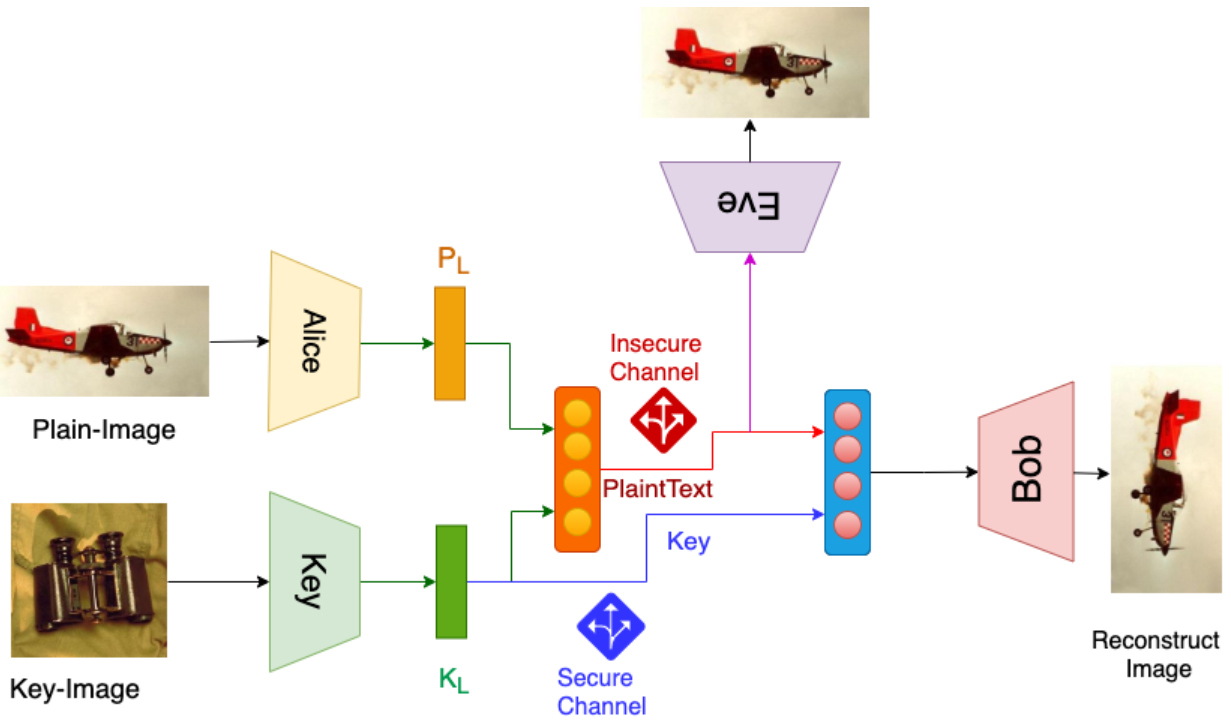
\includegraphics[width=0.90\textwidth]{img/ch3m4.png} 
\caption{CryptoNets 的模式图}
\label{Test}
\end{figure}

\subsection{CryptoNN}

CryptoNN 为以自身研究所开发的神经网路结合功能性加密的演算法,在神经网路领域方面,其架构如图所示,该研究的论文作者表示此类型的加密演算法适用所有神经网路架构,同时在论文中采用以 CNN 改写的架构进行,而在此架构中,使用的演算法为自行开发的功能性加密技术 (Functional Encryption; FE),并于之后并加入安全矩阵运算 (Secure Matrix Computation),其算法与架构如图所示。

\begin{figure}[htb]
\centering 
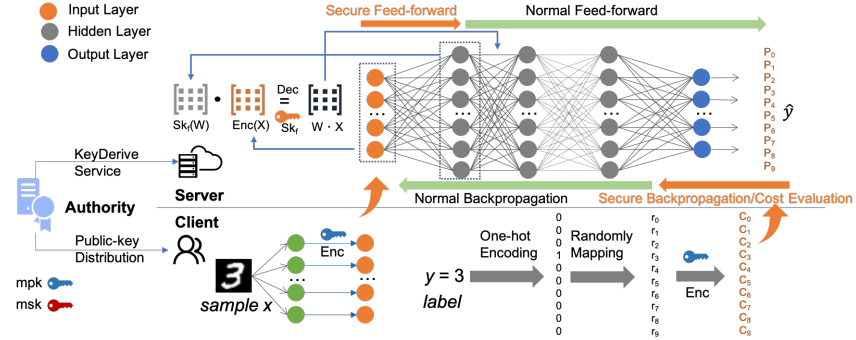
\includegraphics[width=0.90\textwidth]{img/ch3m5.png} 
\caption{CryptoNN 架构}
\label{Test}
\end{figure}

\begin{figure}[htb]
\centering 
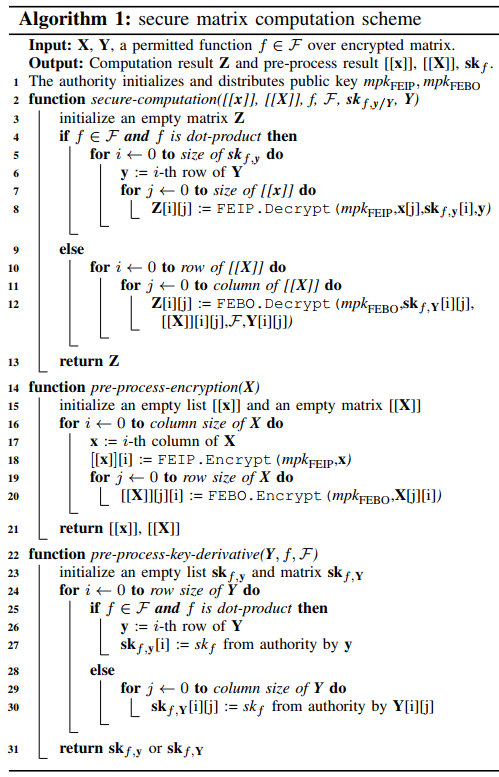
\includegraphics[width=0.90\textwidth]{img/ch3m6.png} 
\caption{CryptoNN 算法}
\label{Test}
\end{figure}
\subsection{CV-QNN}

CV-QNN 结合了量子电脑、类神经网路与加密演算法的概念,十分先进。但由于目前量子电脑技术尚未成熟,故仍暂时无法实作,而只能模拟的方式。其 CV-QNN 的发明是因应量子电脑的产生,可能会对于传统加密演算法产生不小的冲击。在该篇研究中,提及的 CV-QNN 架构如下图所示。其主要构造较近似于 RSA 加密,只是加密与解密的主要机制需要依靠量子电脑运算,同时配合类神经网路相关演算法,可以有效阻挡攻击者以暴力方式破解密码而获取资料。此型态在资安上为一新趋势,或许,在不远的未来,也可以和经生物学或基因与蛋白质的 Encoding 结合,发展出另一些新型态的加密技术,保障使用者的资料安全。

\begin{figure}[htb]
\centering 
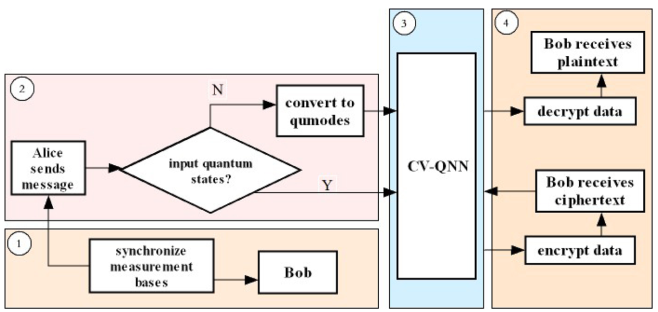
\includegraphics[width=0.90\textwidth]{img/ch3m7.png} 
\caption{CV-QNN}
\label{Test}
\end{figure}